\documentclass[12pt]{article}
\pagestyle{empty}
\usepackage{amsmath,times,bm,hyperref}
\usepackage{amssymb}
\usepackage{graphicx}
\usepackage{listings}
\usepackage{xcolor}
\lstset { %
    language=C++,
    backgroundcolor=\color{black!5}, % set backgroundcolor
    basicstyle=\footnotesize,% basic font setting
}

%%%%%%%%%%%%%%%%%%%%%%%%%%%%%%%%%%%%%%%%%%%%%%%%%%
% Do not modify the dimensions of the page
\setlength{\topmargin}{0mm}
\setlength{\headheight}{0mm}
\setlength{\headsep}{0mm}
%% 25.4 -25.4 = 0
\setlength{\topmargin}{0mm}
%% 25.4 -25.4 = 0
\setlength{\oddsidemargin}{0mm}
%% 210 -25(left) -25(right) = 160
\setlength{\textwidth}{160mm}
%% 297 -25(top) -30(bottom) = 242
\setlength{\textheight}{242mm}
\setlength{\parindent}{0pt}
\setlength{\parskip}{12pt}
% Do not modify the dimensions of the page
%%%%%%%%%%%%%%%%%%%%%%%%%%%%%%%%%%%%%%%%%%%%%%%%%%

\begin{document}

\begin{center}
% TITLE: replace text with your abstract title WITHOUT full stop
\textbf{\Large
Homework 6
}\\
\normalsize Due May 27 2021

% AUTHOR/AFFILIATION: handled by authblk. 
% Use only one of the two following methods for author listing. Delete or comment out the other.
% Add/remove authors/affiliations as necessary, complete following the template without adding additional superscript/footnotes  

% 1- Authors have the same affiliation:
% ~~~~~~~~~~~~~~~~~~~~~~~~~~~~~~~~~~~~


%%%%% AFFILIATIONS %%%%%

\end{center}
\begin{enumerate}
\item Calculate the constraint ratio of the elements shown in Figure \ref{fig:elem} and make comments.


\begin{figure}[h]
	\begin{center}
	\begin{tabular}{c}
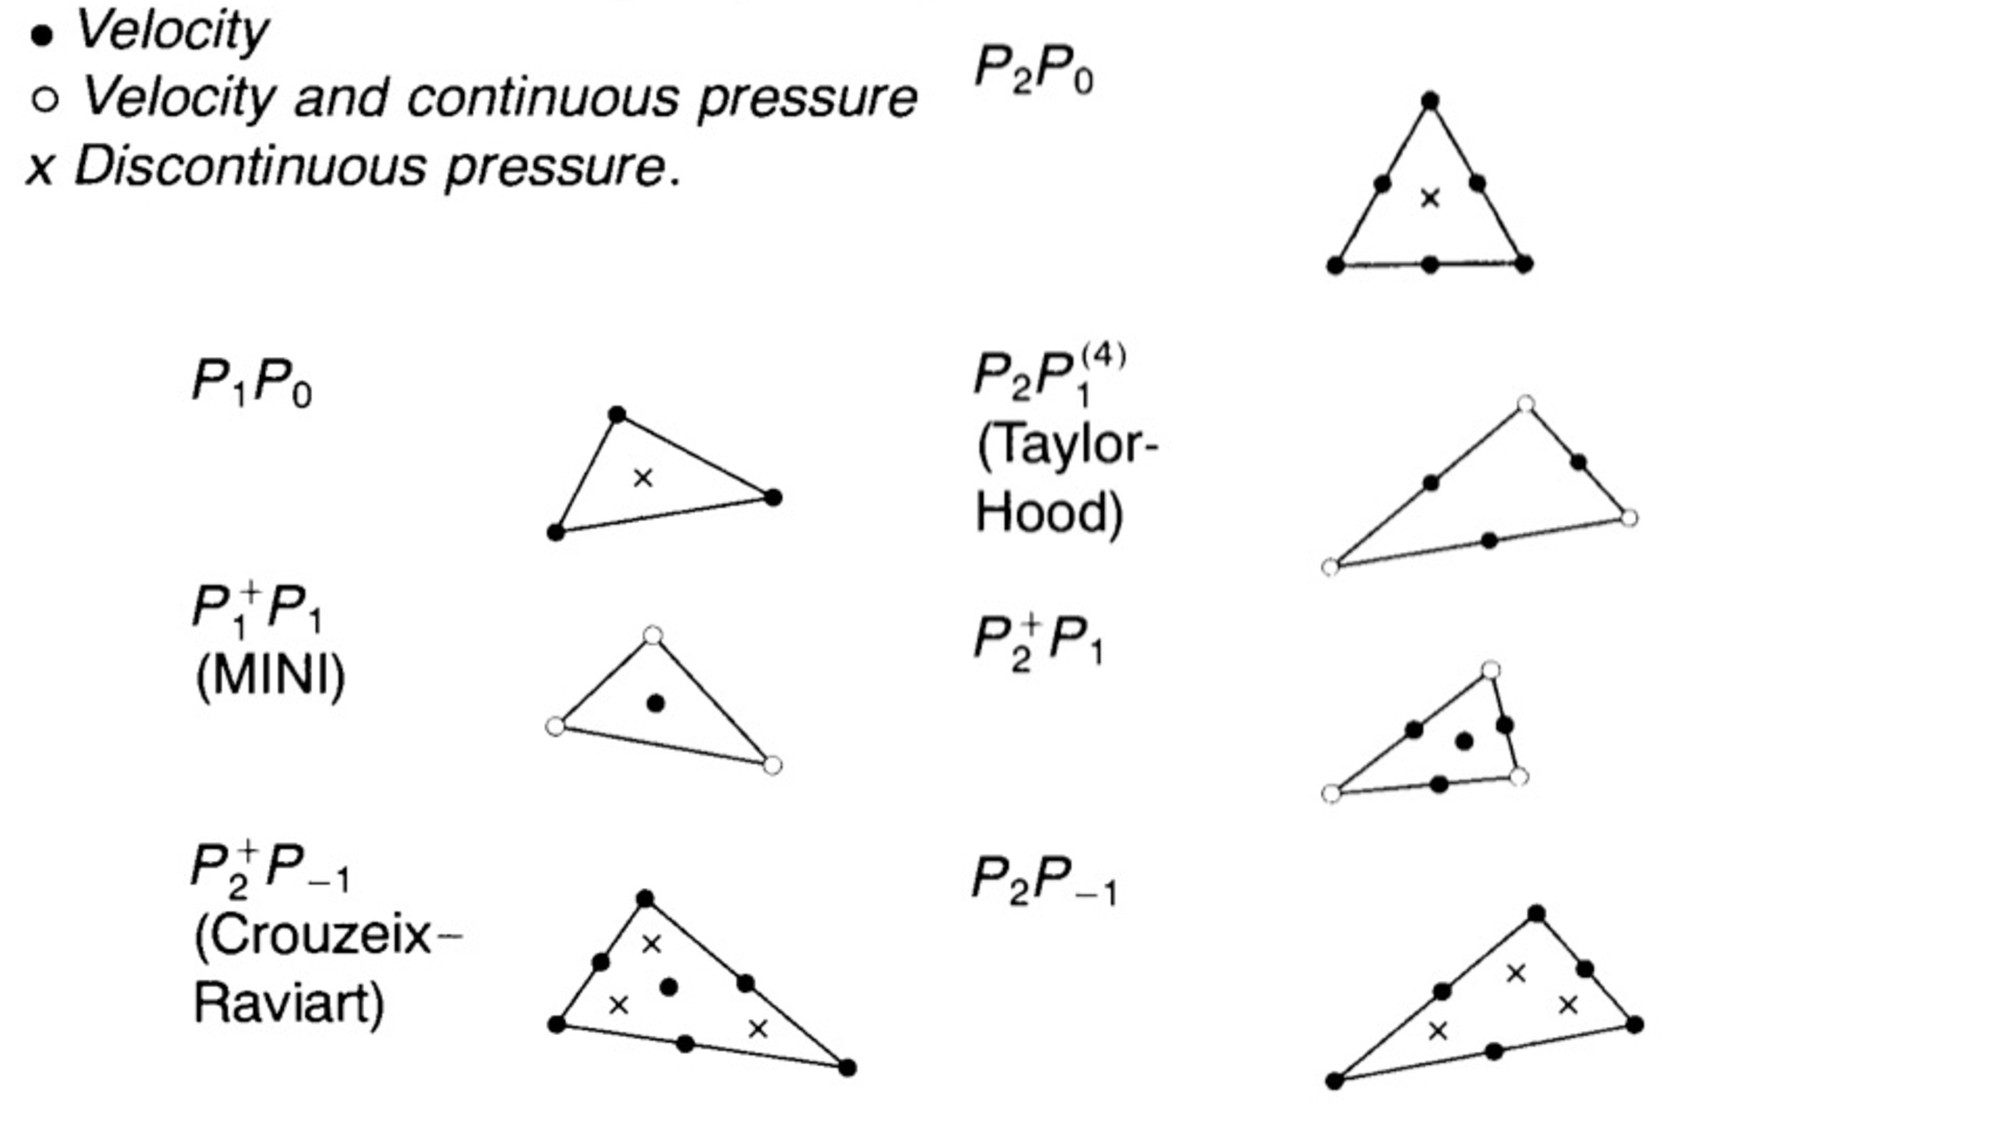
\includegraphics[angle=0, trim=0 0 0 0, clip=true, scale = 0.35]{./element1.pdf}\\
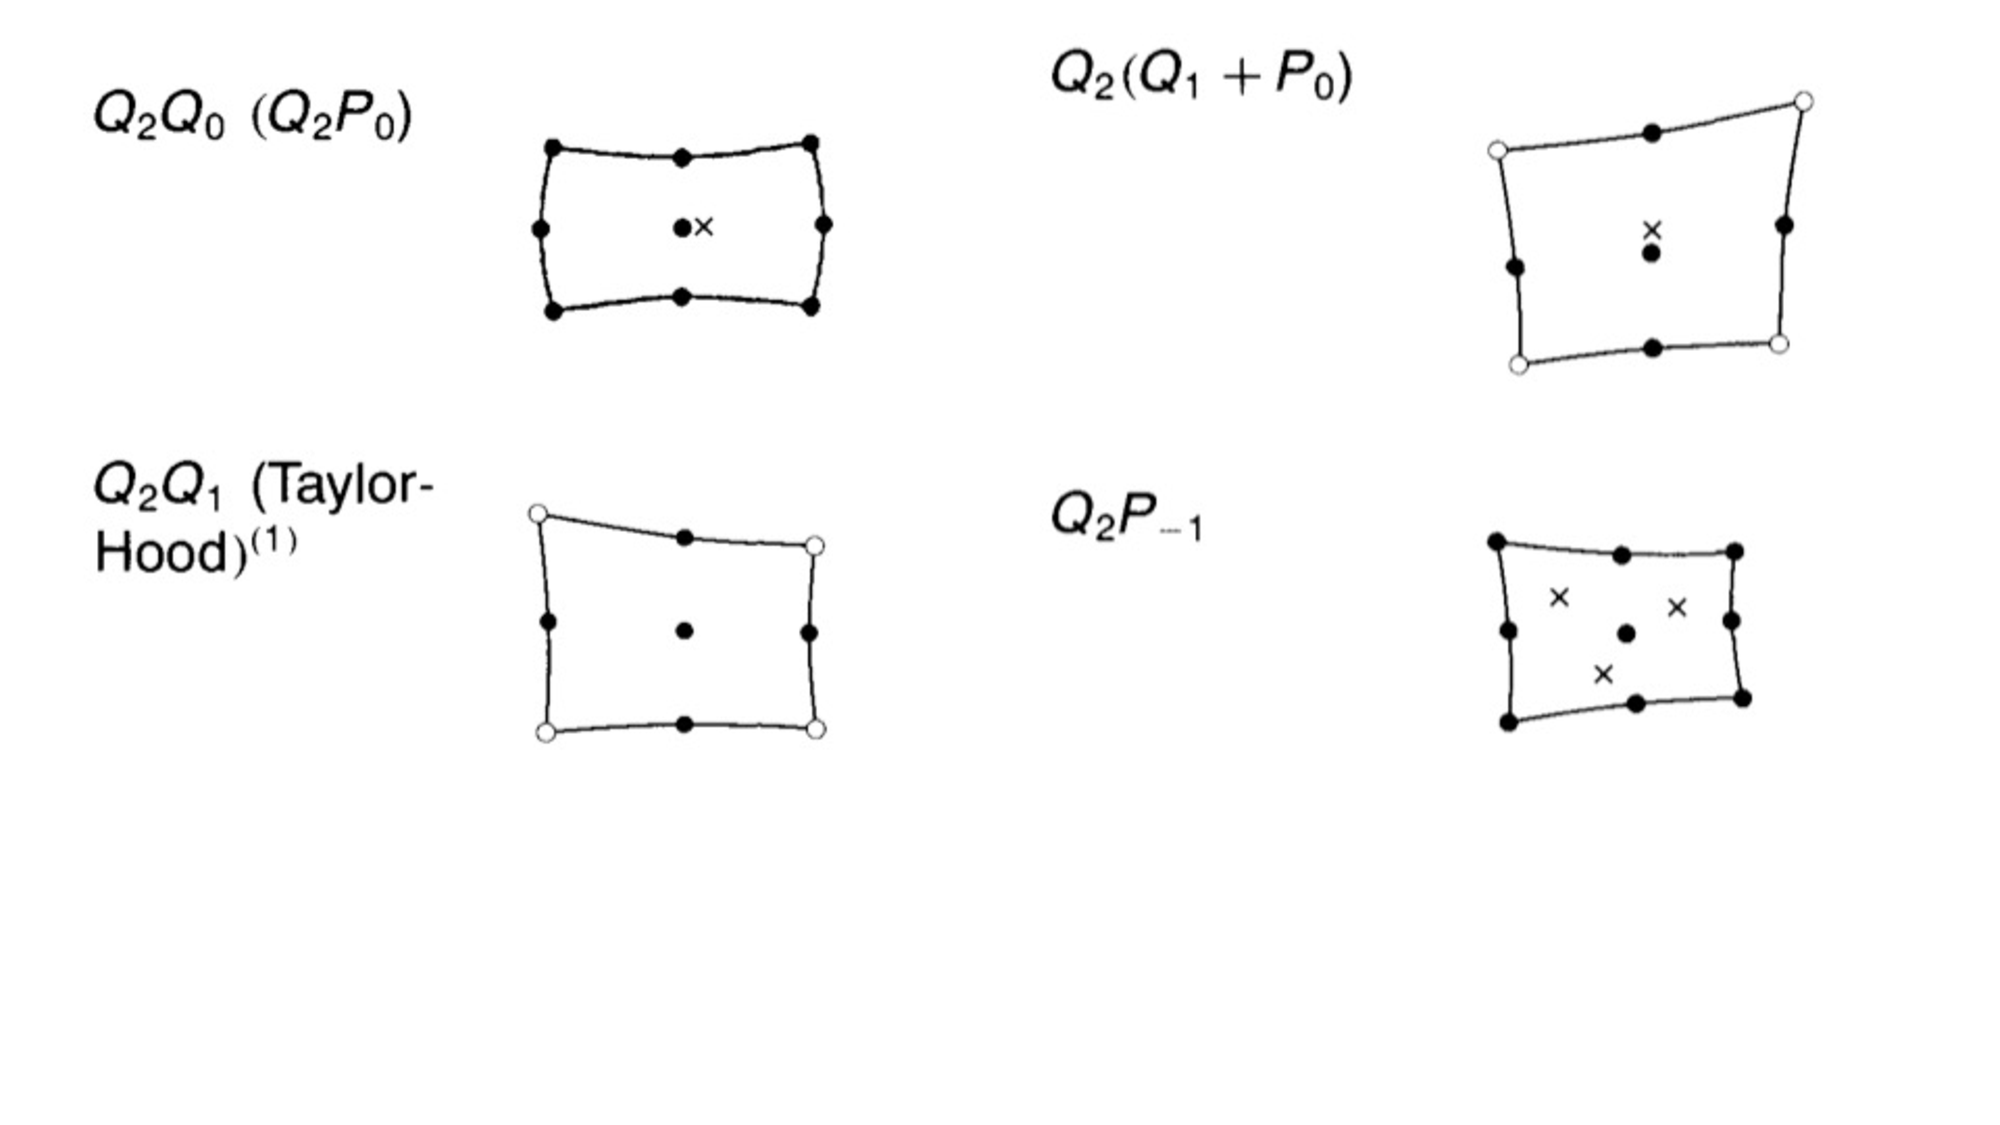
\includegraphics[angle=0, trim=0 150 0 0, clip=true, scale = 0.35]{./element2.pdf}
\end{tabular}
\end{center} 
\caption{A list of 2D mixed elements}
\label{fig:elem}
\end{figure}


\item Hughes FEM book, page 428, exercise 3.

\item Hughes FEM book, page 428, exercise 4.

\item Hughes FEM book, page 473, exercise 2.

\item Hughes FEM book, page 498, exercise 4.

\item Hughes FEM book, page 501, exercise 5.

\item Hughes FEM book, page 502, exercise 7.

\item Hughes FEM book, page 542, exercise 16. Submit your code as well.



\end{enumerate}

\end{document}

